\chapter{System Description}
The Surface Vessel at hand is a complex system composed by several subsystems. These are shown in \autoref{fig:systemDiagram}, in which the link between the different subsystems is also depicted.
\begin{figure}[H]
    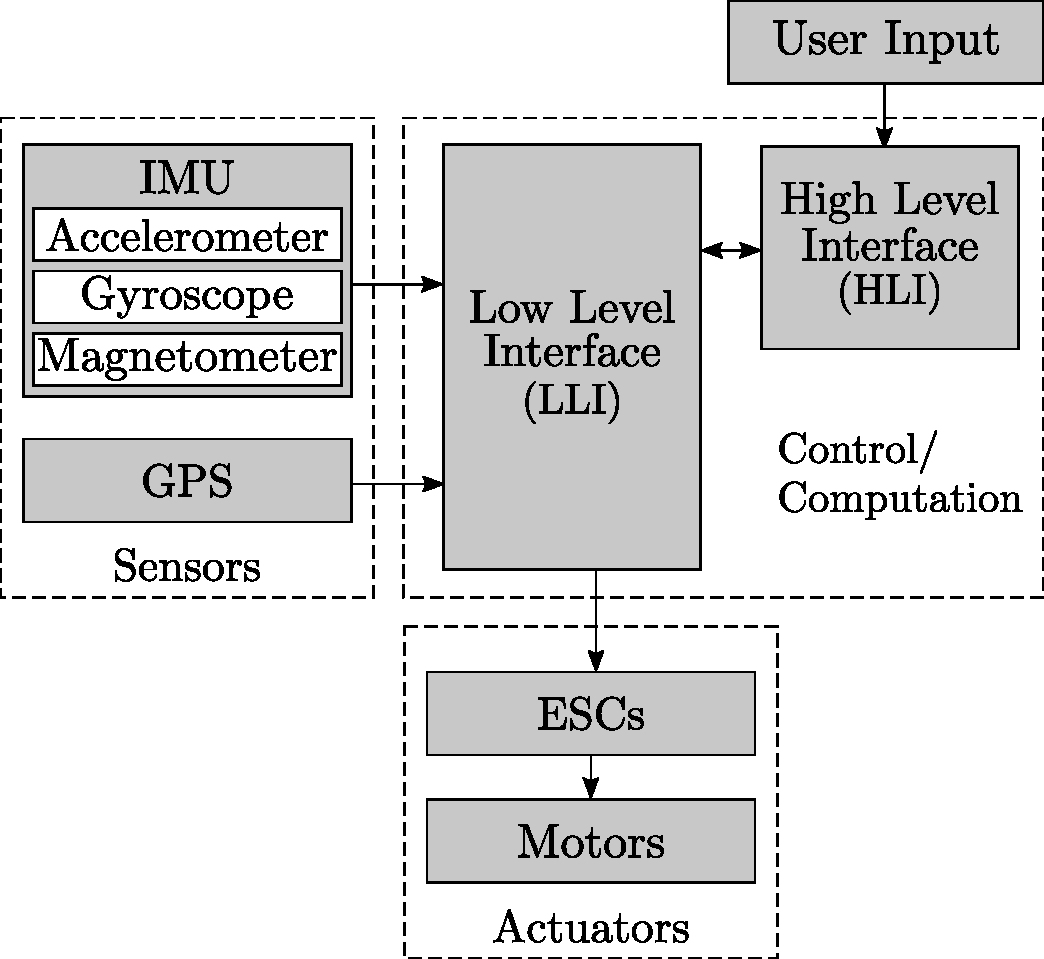
\includegraphics[width=0.6\textwidth]{figures/systemDiagram}
    \caption{}
    \label{fig:systemDiagram}
\end{figure}
The main parts of the system are the actuation, the sensors and the control units, see \autoref{fig:systemDiagram}. The control unit gathers information from the sensors, in particular, the IMU and the GPS. This is done by the Low Level Interface which then sends it to the high level interface where the control algorithms run. The calculated actuation action is then sent back to the Low Level Interface that sends the command to the actuation system. The ESCs calculate then the required signal to make the motors turn at the right speed. 

This chapter describes briefly the main components of the surface vessel used in this project. \cite{aauship}

